\documentclass[12pt,preprint]{aastex}

\newcommand{\vdag}{(v)^\dagger}
\newcommand{\myemail}{skywalker@galaxy.far.far.away}
\slugcomment{Draft version}
 
\shorttitle{A Study of the Point Spread Function at SDSS}
\shortauthors{Xin, Ivezi\'{c} and Friends}
 
\begin{document}

\title{A Study of the Point Spread Function in SDSS Images}    %line break \\ is allowed in title

\author{B. Xin$^1$, \v{Z}. Ivezi\'{c}$^2$, R.H. Lupton$^3$, P. Yoachim$^2$, R.L. Jones$^2$, C. Claver$^1$, G. Angeli$^1$}
\and
\author{Other Contributors}

\affil{$^1$Large Synoptic Survey Telescope, Tucson, AZ 85719}
\affil{$^2$Department of Astronomy, University of Washington, Seattle, WA 98195}
\affil{$^3$Department of Astrophysical Sciences, Princeton University, Princeton, NJ 08544}

\begin{abstract}
We use SDSS imaging data in $ugriz$ passbands to study the shape of
point spread function (PSF) profile and the variation of its width with 
wavelength and time. We find that the PSF profile is well described by 
theoretical predictions based on von Karman's turbulence theory and
can be parametrized by a single parameter, the profile's FWHM (full width
at half maximum). The profile shape is very similar to the ``double gaussian
plus power-law wing'' decomposition used by SDSS, but here it is modeled 
with a single free model parameter, rather than six as in SDSS pipeline. 
The FWHM variation with wavelength folows the
$\lambda^{-0.3}$ power law. We also measure the temporal and angular
structure functions for FWHM and find lots of interesting results \dots
\end{abstract}

\keywords{imaging point spread function --- SDSS}
 
\section{Introduction}


% \section{Introduction}

ZI write a brief overview of SDSS and motivation for analysis (e.g. performance optimization
for LSST, \citealt{LSSToverview}): this shouldn't be hard and can be done in about a day. 

Hey Bo! Here is an example of using bibtex and cite call: SDSS PSF algorithm is described 
in \cite{Lupton2001}, \cite{Lupton2002}, and \citet[][see \S4.3]{SDSSEDR}.

Bo or ZI: add a brief summary with a few references (e.g. Young, Tyson, Roddier,
Tokovinin papers; can also recruit George for this part!) about what is known 
regarding:  PSF profile shape (e.g. Kolmogorov vs. von Karman), 
the dependence of FWHM on wavelength, and angular and temporal 
structure functions. 

Paper layout here.

  

\section{Data Overview} 


%\section{Data Overview} 

We describe here the SDSS dataset and seeing estimates used in this work. The
selected subset of data, the so-called Stripe 82, represents about one third of
all SDSS imaging data. 

\subsection{Stripe 82 dataset} 

The equatorial Stripe 82 region (22$^h$24$^m$ $<$ R.A. $<$ 04$^h$08$^m$, 
$-$1.27$^\circ$  $<$ Dec $<$ $+$1.27$^\circ$, about 
290 deg$^2$) from the southern Galactic cap ($-64^\circ < b <  -20^\circ$) was repeatedly imaged (of order
one hundred times) by SDSS to study time-domain phenomena (such as supernovae, asteroids, variable stars, quasar 
variability).  An observing stretch of SDSS imaging data is called a ``run''. Often there is only a single
run for a given observing night, though sometimes there are multiple
runs per night. In this paper we use seeing data for 
108 runs, with a total of 947,400 fields, obtained between September,
1998 and September 2008 (there are 6 camera columns, each with 5 filters; for more
details please see \citealt{Gunn2006}). All runs are obtained during the Fall observing season (September to 
December). Astrometric and photometric aspects of this dataset have been discussed in detail by 
\cite{Ivezic2007} and \cite{Sesar2007}. 


\subsection{The treatment of seeing in SDSS}
 
Even in the absence of atmospheric inhomogeneities, the SDSS telescope delivers images whose 
FWHMs vary by up to 15\% from one side of a CCD to the other; the worst effects are seen in 
the chips farthest from the optical axis \citep{Gunn2006}. Moreover, since the atmospheric 
seeing varies with time, the delivered image quality is a complex two-dimensional function 
even on the scale of a single field (for an example of the instantaneous image quality across 
the imaging camera, see Figure 7 in \citealt{SDSSEDR}). 
 
The SDSS imaging PSF is modeled 
heuristically in each band using a Karhunen-Lo\'{e}ve (K-L) transform \citep{Lupton2002}. 
Using stars brighter than roughly 20$^{th}$ magnitude, the PSF images from a series of five 
fields are expanded into eigenimages and the first three terms are kept (K-L transform is 
also known as the Principal Component Analysis). The angular variation of the eigencoefficients
is fit with polynomials, using data from the field in question, plus the immediately preceding 
and following half-fields. The success of this K-L expansion is gauged by comparing PSF 
photometry based on the modeled K-L PSFs with large-aperture photometry for the same 
(bright) stars \citep{SDSSEDR}. 
Parameters that characterize seeing for one field of imaging data are stored in the so-called psField 
files\footnote{https://data.sdss.org/datamodel/files/PHOTO\_REDUX/RERUN/RUN/objcs/CAMCOL/psField.html}. 
The status parameter flag for each field indicates the success of the K-L decomposition.

In addition to the K-L decomposition, the SDSS processing pipeline computes parameters of the 
best-fit circular double Gaussian, evaluated at the center of each field. The measured PSF profiles are 
extended to $\sim$30 arcsec using observations of bright stars and at such large radii 
double Gaussian fits underpredict the measured profiles. For this reason, the fits are extended 
to include the so-called ``power-law wings'', which is reminiscent of
the Moffat function,
\begin{equation}
\label{eq:SDSSPSF}
        PSF(r) = {\exp(-{r^2\over 2\,\sigma_1^2}) + b\,\exp(-{r^2\over 2\,\sigma_2^2})
           + p_0\left(1 + { r^2 \over \beta \sigma_P^2}\right)^{-\beta/2} \over 1 + b + p_0}.
\end{equation} 
The measured PSFs are thus modeled using 6 free parameters ($\sigma_1$, $\sigma_2$, $\sigma_P$,
$b$, $p_0$ and $\beta$), and the best-fit parameters are reported in the psField files. 
Given that the measured profiles include only up to 10 data points, the fits are usually excellent
although they do not appear very robust (for examples of bad fits see Sec.~\ref{sec:psffit}).
%Fig.~\ref{fig:psffit}). 

 


\section{The PSF profile analysis}

Compare to SDSS, emphasize superiority of 1 parameter vs. 6 parameters fit

Discuss profile shape stability when the seeing is rapidly  changing 

\begin{figure}
\centering
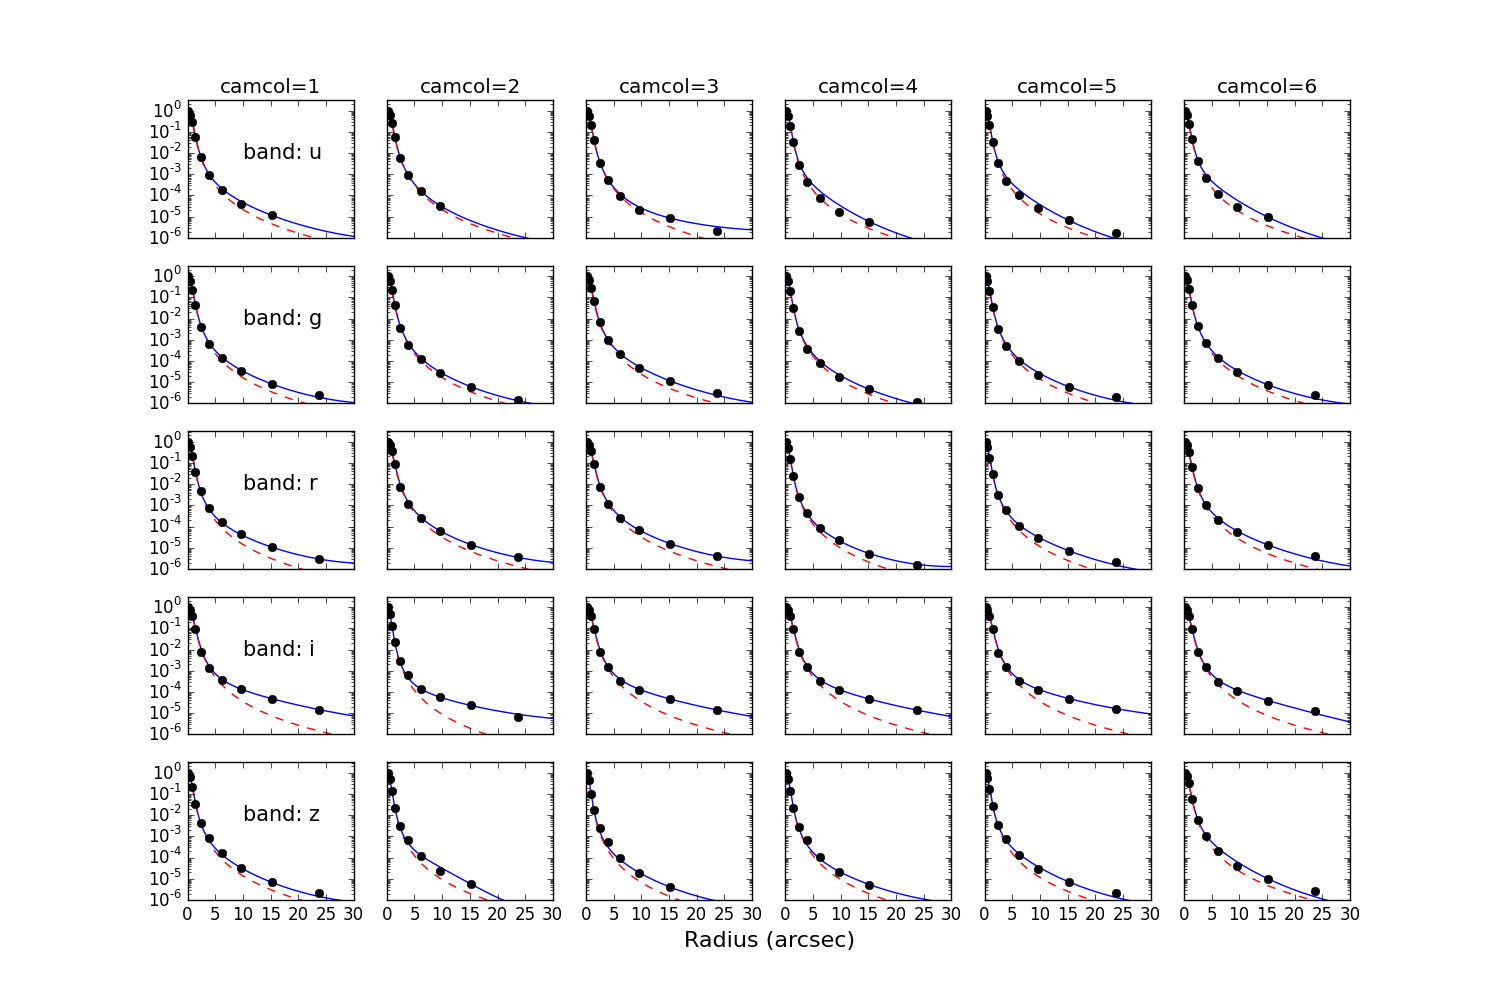
\includegraphics[width=0.9\textwidth]{FIGURES/psffit.png}
\caption{Fit to the PSF profiles from run 1033, field 200. Red curves
  are results of 1-parameter von Karman fits. Blue curves are red
  curve convolved with the instrument PSF, where the scaling factor on
  the tail component is allowed to vary.
\label{fig:psffit}}
\end{figure}

\section{The analysis of FWHM behavior} 

Now that we understand (heopfully) that the seeing is by and large described by 
a single parameter, FWHM, we study three aspects of its variation, as follows.


\subsection{The FWHM dependence on wavelength} 

Asumming a power law, FWHM$\propto \lambda^{-\alpha}$, what can we say 
about $\alpha$ distribution? 

\begin{figure}
\centering
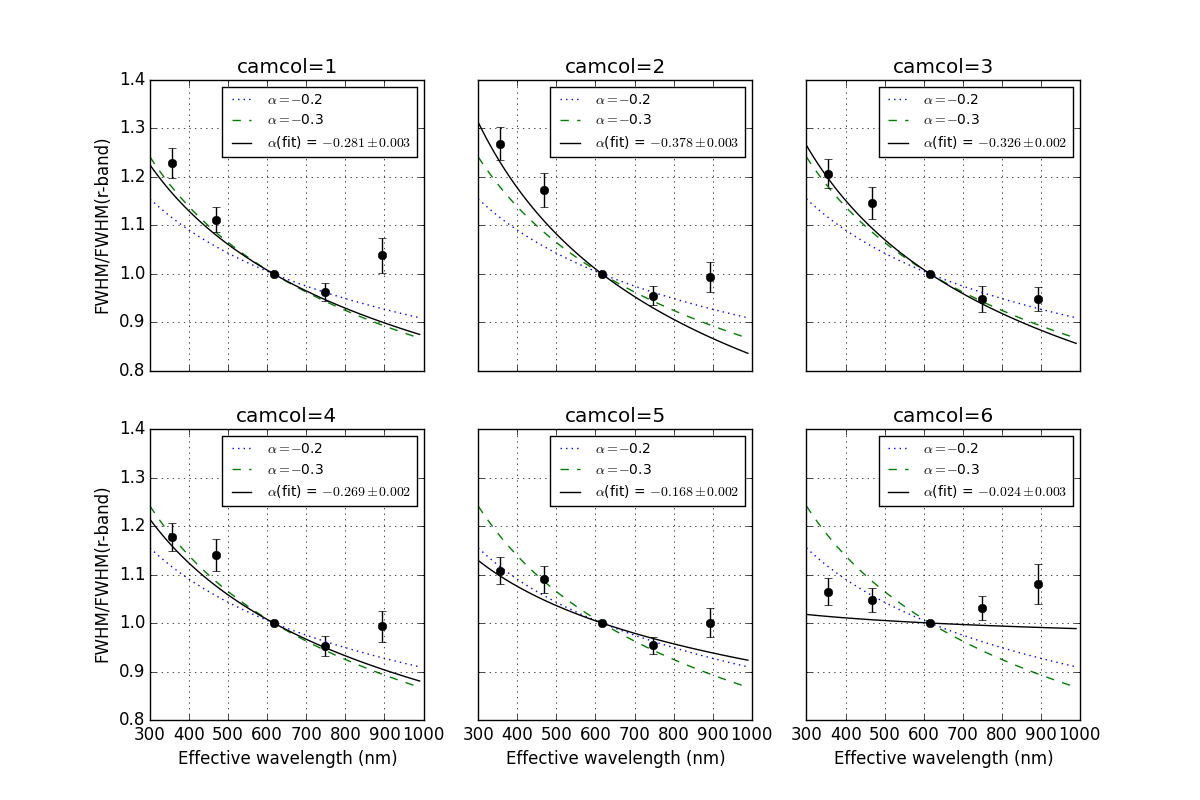
\includegraphics[width=0.9\textwidth]{FIGURES/fwhm_lambda.png}
\caption{FWHM as functions of wavelength for run 3427.
\label{fig:fwhm_lambda}}
\end{figure}

\begin{figure}
\centering
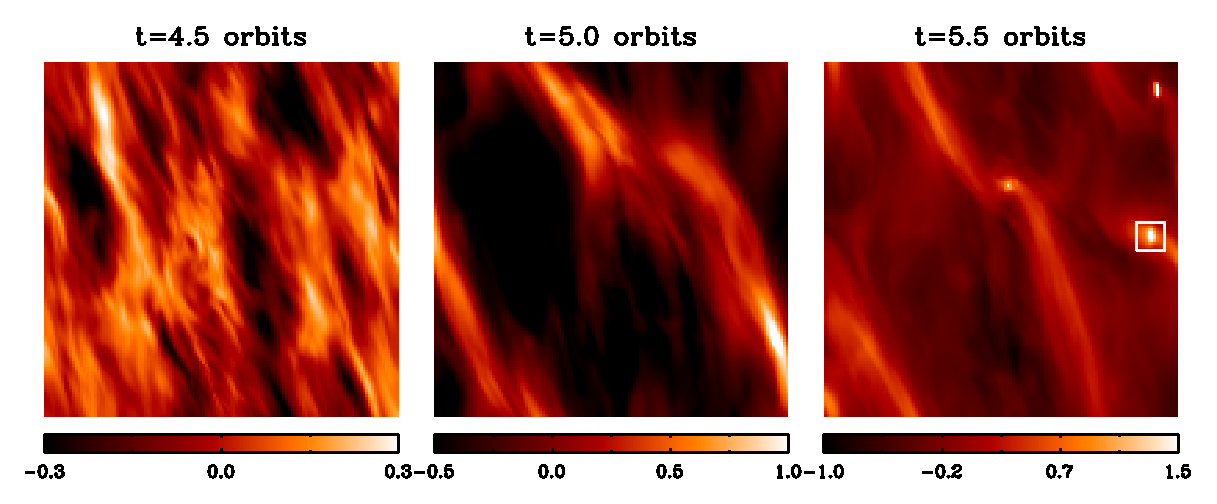
\includegraphics[width=0.9\textwidth]{FIGURES/f3.eps}
\caption{statistics for $\alpha$ from all 109 runs.
\label{fig:alpha_stat}}
\end{figure}


Why is SDSS PSF different for the $i$ band? The $i$ band psf has ``stronger tails''
becuse of scattering in the CCD.  The Si is transparent at long $i$-band wavelengths 
so light goes all the way through the chip and is reflected off the solder, and passes 
back up through the Si. This effect is not visible in the $z$ band because in this case
thick front-side chips are used (in all other bands, thin back-side chips are used). 


\subsection{Angular structure function} 

Cross-correlation of FWHM for 6 camera columns and the measurement of the angular
structure function (that is, the covariance vs. angular distance). 

\begin{figure}
\centering
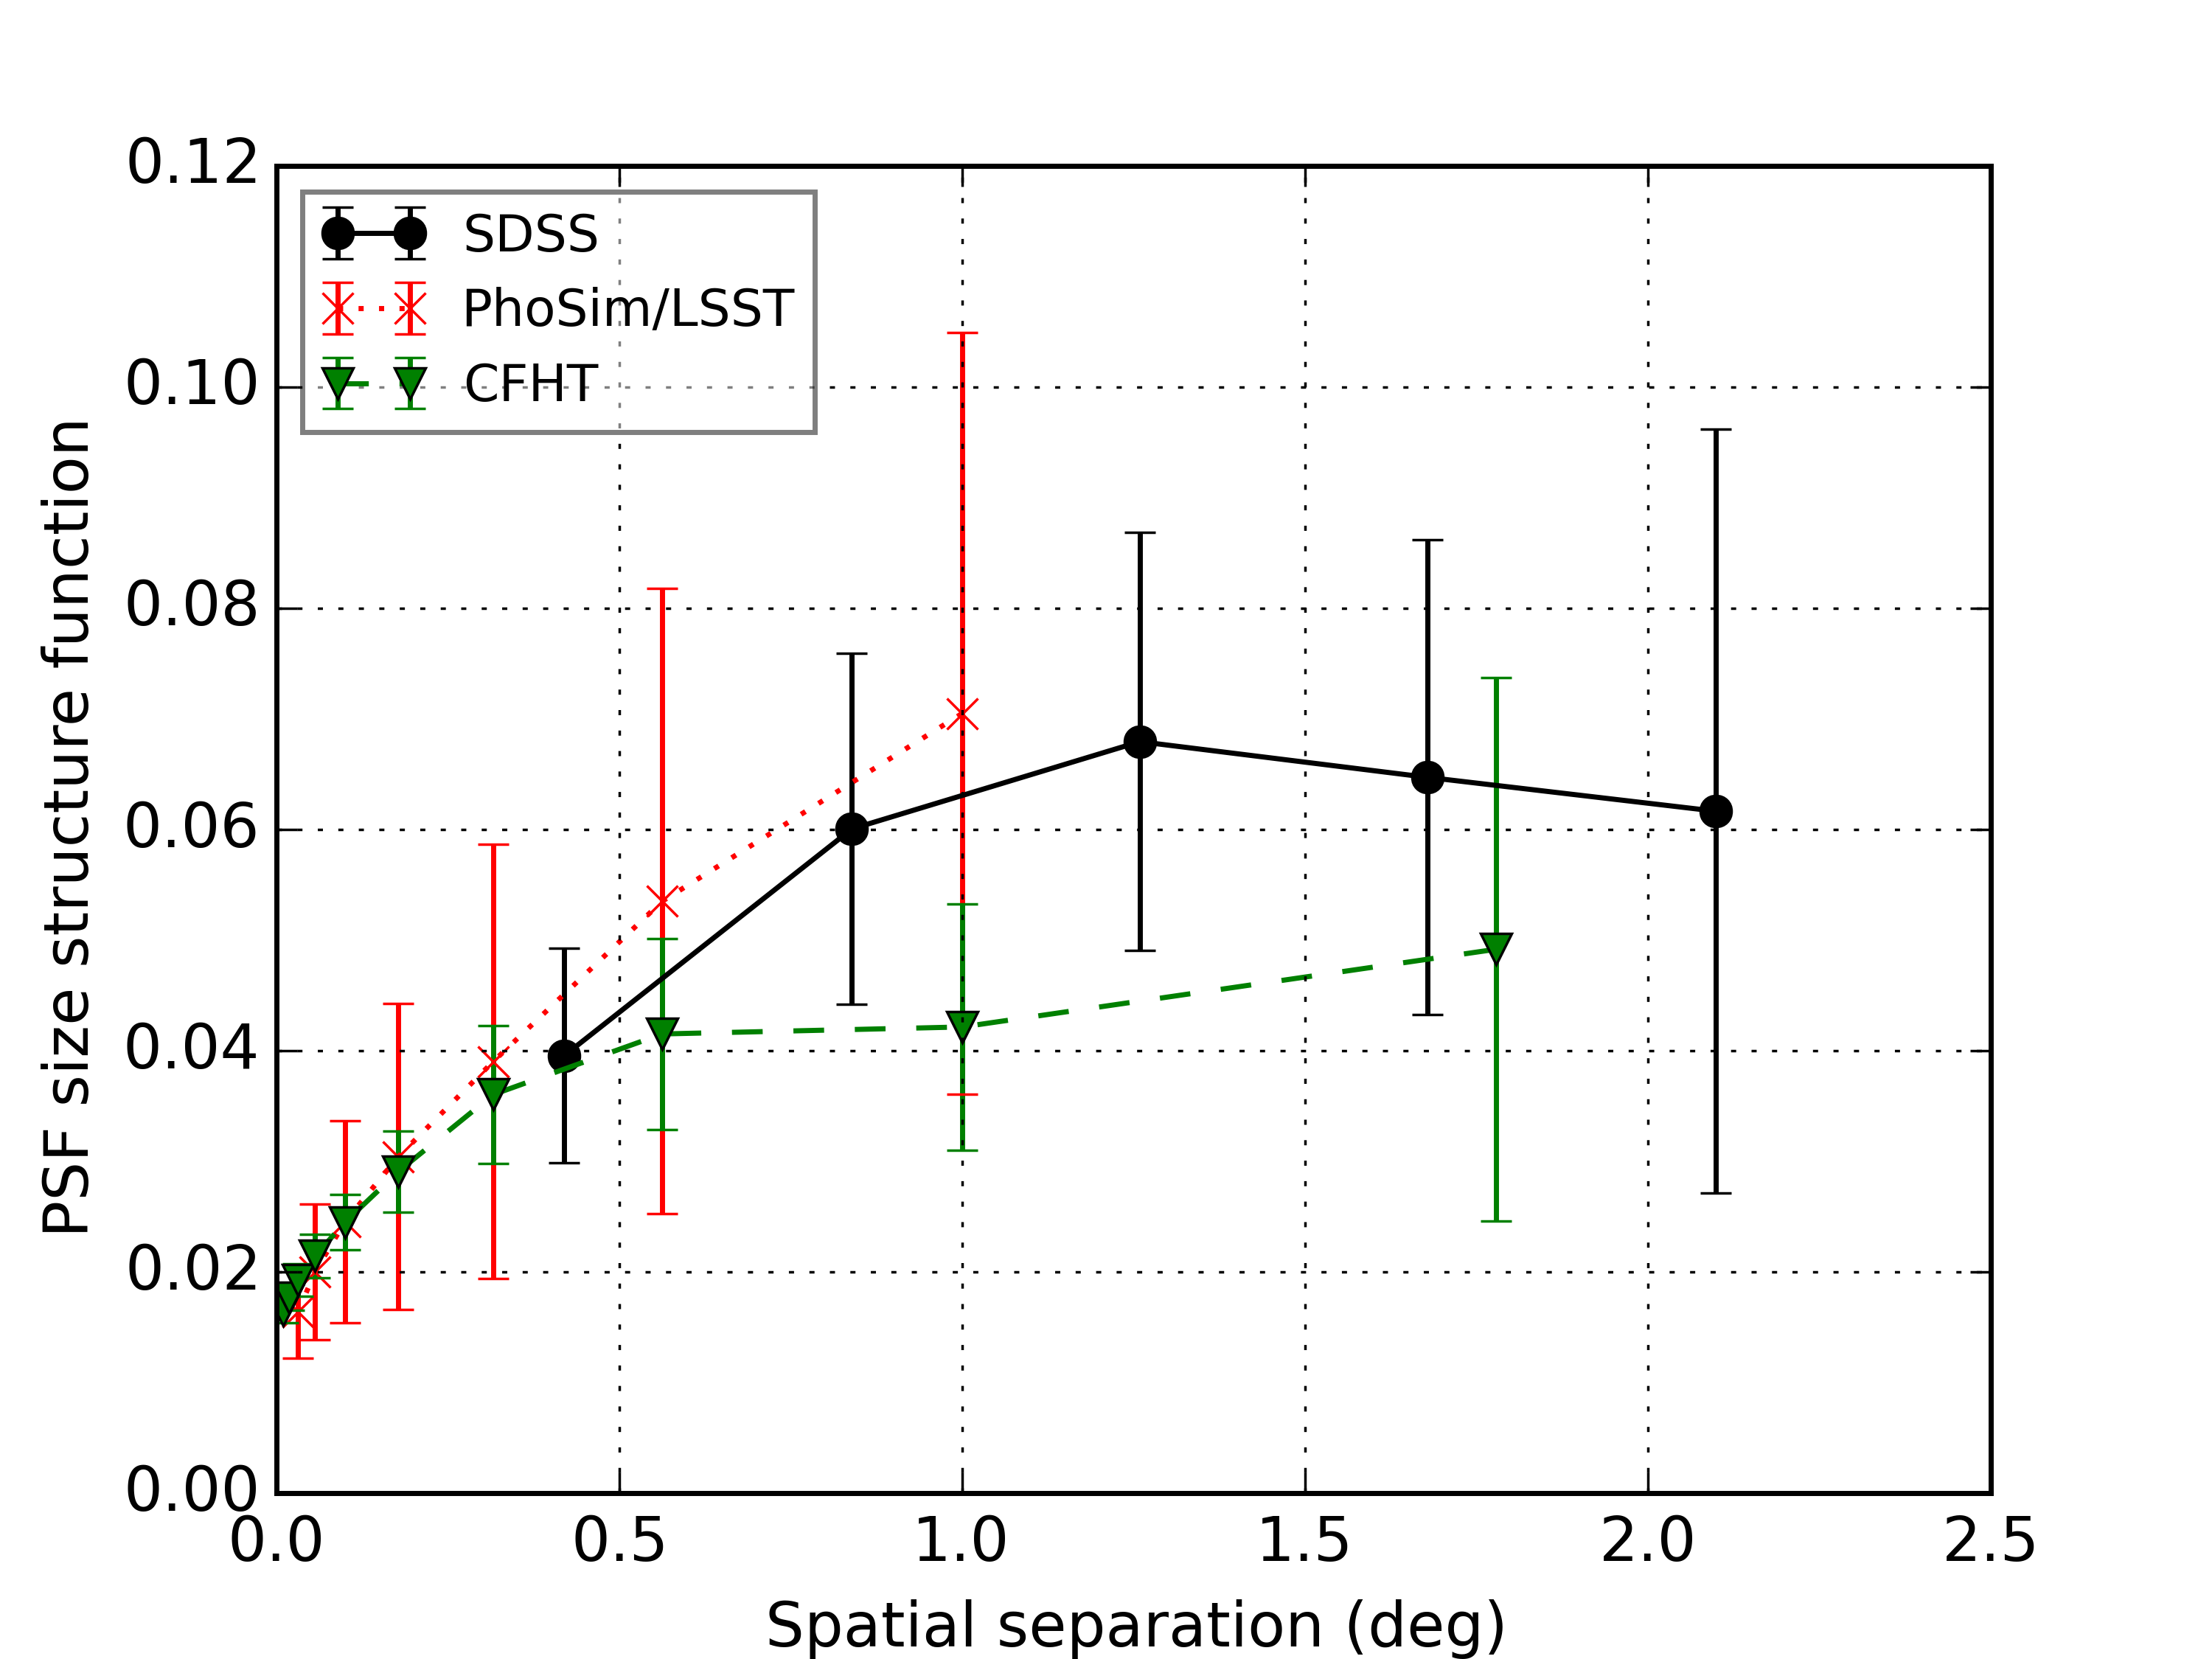
\includegraphics[width=0.9\textwidth]{FIGURES/spatial.png}
\caption{spatial correlation for run 1009. 
\label{fig:fwhm_lambda}}
\end{figure}

\begin{figure}
\centering
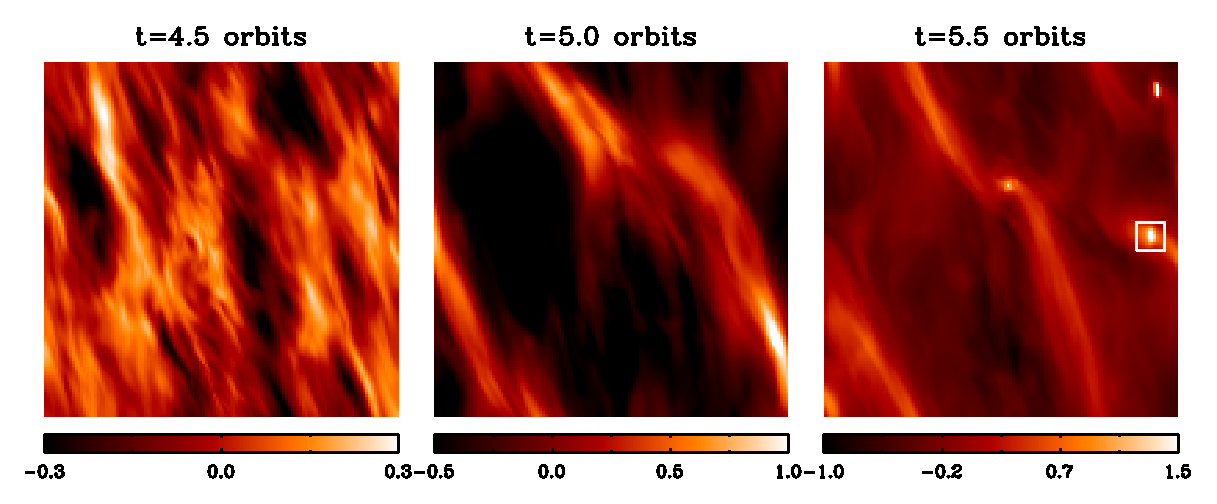
\includegraphics[width=0.9\textwidth]{FIGURES/f3.eps}
\caption{statistics for correlation coefficients from all 109 runs.
\label{fig:alpha_stat}}
\end{figure}


\subsection{Temporal auto-correlation function}

Study the temporal power spectrum:
\begin{itemize}
\item Let's start with plain Fourier transform and look at power spectra (we can 
    play games with co-addition, 6 columns for a given run, or all runs)
\item Potentially, we could also look at  Kelly and Becker code  (2014, ApJ 788, 33) 
\item Here we can compare to Chuck's CP measurements (in opsim db) 
\end{itemize} 

\begin{figure}
\centering
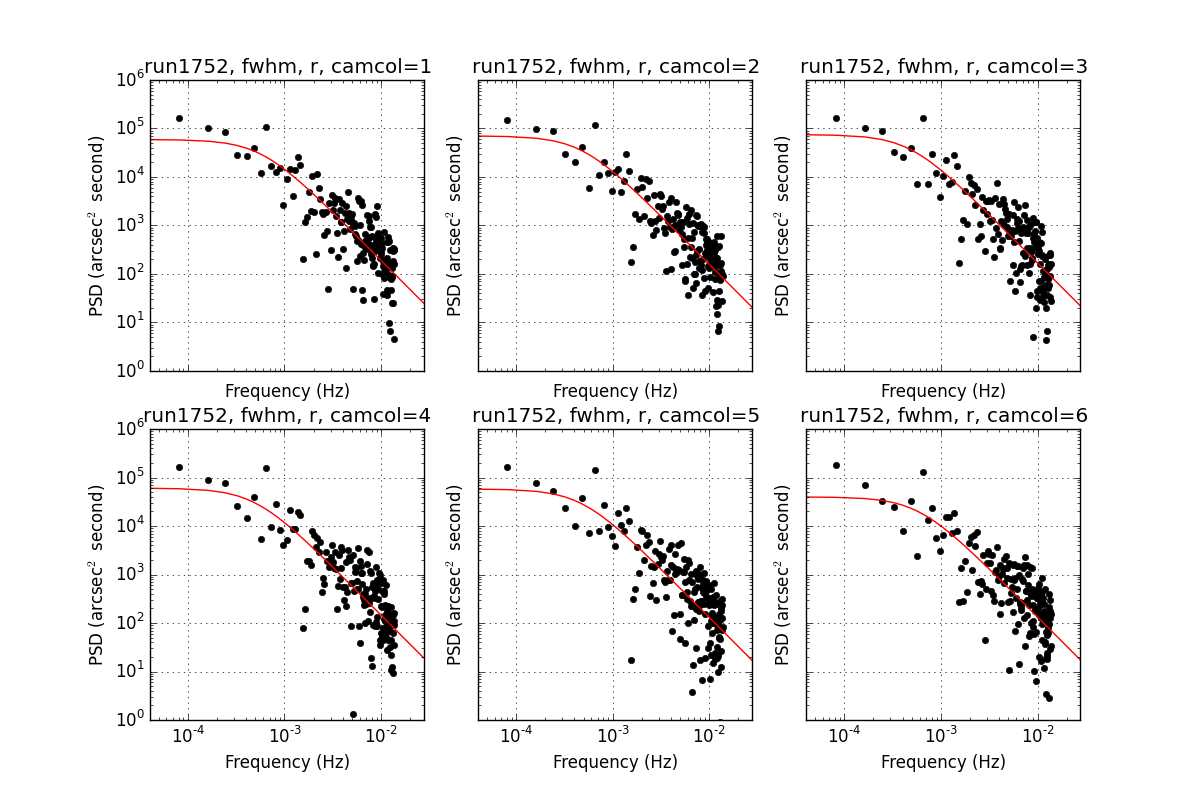
\includegraphics[width=0.9\textwidth]{FIGURES/temporal.png}
\caption{spatial correlation for run 1752. Average
  $f_0 = 5.1\times 10^{-4} Hz$, Average $\tau = 314 sec.$ 
\label{fig:psd}}
\end{figure}

\begin{figure}
\centering
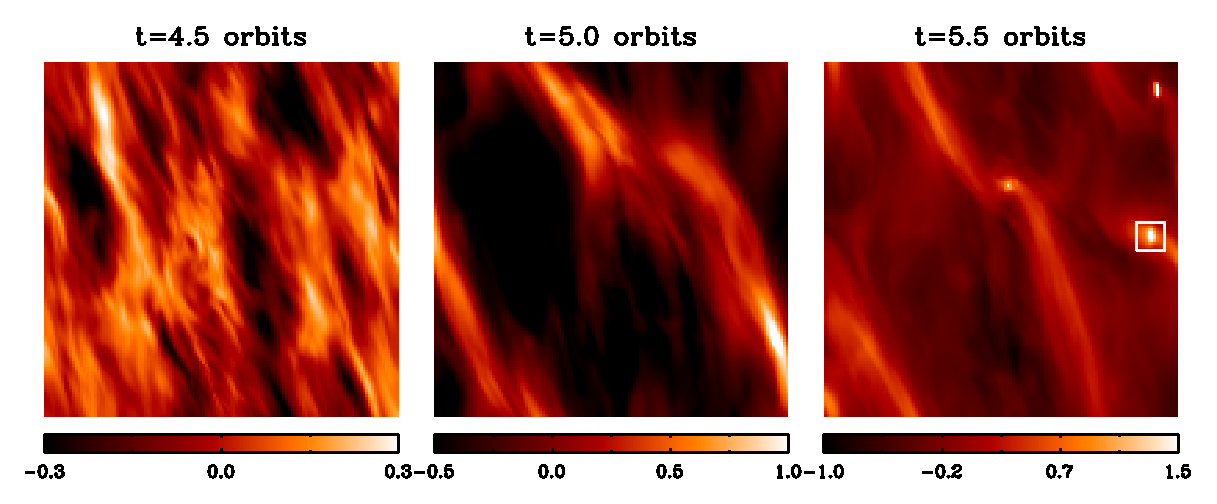
\includegraphics[width=0.9\textwidth]{FIGURES/f3.eps}
\caption{statistics for correlation coefficients from all 109 runs.
\label{fig:psd_stat}}
\end{figure}



\begin{table}[t!]
\caption{A little stolen table to test if it works here... It does! }
\vskip 0.05in
\begin{tabular}{|l|c|c|c|c|c|}
\hline  
    $r$   &  $\sigma^a_{xy} $  & $\sigma^b_\pi$  &   $\sigma^c_\mu$   &  $\sigma^d_1$  &  $\sigma^e_C$  \\
    mag &       mas            &      mas  & mas/yr &   mag   &    mag  \\
\hline  
       21 &  11  &  0.6  &  0.2   &   0.01  &   0.005 \\
       22 &  15  &  0.8  &  0.3   &   0.02  &   0.005 \\
       23 &  31  &  1.3  &  0.5   &   0.04  &   0.006 \\
       24 &  74  &  2.9  &  1.0   &   0.10  &   0.009 \\
\hline                         
\end{tabular}
\\ \vskip 0.05in
  $^a$ Typical astrometric accuracy (rms per coordinate per visit); \\
  $^b$ Parallax accuracy for 10-year long survey; \\
  $^c$ Proper motion accuracy for 10-year long survey; \\
  $^d$ Photometric error for a single visit (two 15-second exposures); \\
  $^e$ Photometric error for coadded observations (see Table 1). \\
\end{table}


\acknowledgments
We are grateful to George A. for buying us tamales and drinks. 


%% To help institutions obtain information on the effectiveness of their
%% telescopes, the AAS Journals has created a group of keywords for telescope
%% facilities. A common set of keywords will make these types of searches
%% significantly easier and more accurate. In addition, they will also be
%% useful in linking papers together which utilize the same telescopes
%% within the framework of the National Virtual Observatory.
%% See the AASTeX Web site at http://aastex.aas.org/
%% for information on obtaining the facility keywords.

%% After the acknowledgments section, use the following syntax and the
%% \facility{} macro to list the keywords of facilities used in the research
%% for the paper.  Each keyword will be checked against the master list during
%% copy editing.  Individual instruments or configurations can be provided 
%% in parentheses, after the keyword, but they will not be verified.

{\it Facilities:} \facility{SDSS}, \facility{LSST}.

%% Appendix material should be preceded with a single \appendix command.
%% There should be a \section command for each appendix. Mark appendix
%% subsections with the same markup you use in the main body of the paper.

%% Each Appendix (indicated with \section) will be lettered A, B, C, etc.
%% The equation counter will reset when it encounters the \appendix
%% command and will number appendix equations (A1), (A2), etc.

%\appendix
%
%\section{Appendix material}

%% The reference list follows the main body and any appendices.
%% Use LaTeX's thebibliography environment to mark up your reference list.
%% Note \begin{thebibliography} is followed by an empty set of
%% curly braces.  If you forget this, LaTeX will generate the error
%% "Perhaps a missing \item?".
%%
%% thebibliography produces citations in the text using \bibitem-\cite
%% cross-referencing. Each reference is preceded by a
%% \bibitem command that defines in curly braces the KEY that corresponds
%% to the KEY in the \cite commands (see the first section above).
%% Make sure that you provide a unique KEY for every \bibitem or else the
%% paper will not LaTeX. The square brackets should contain
%% the citation text that LaTeX will insert in
%% place of the \cite commands.

%% We have used macros to produce journal name abbreviations.
%% AASTeX provides a number of these for the more frequently-cited journals.
%% See the Author Guide for a list of them.

%% Note that the style of the \bibitem labels (in []) is slightly
%% different from previous examples.  The natbib system solves a host
%% of citation expression problems, but it is necessary to clearly
%% delimit the year from the author name used in the citation.
%% See the natbib documentation for more details and options.


\bibliographystyle{aj}
\bibliography{sdsspsf}


%% The following command ends your manuscript. LaTeX will ignore any text
%% that appears after it.

\end{document}

%%
%% End of file `sample.tex'.

----------Completed: ----------------

ZI:  find exact definition of neff_psf (is it based on fit or input data?) 
Bo: add analysis directory and py code 


1)  make files, one per run, as a function of field number, with
- field, camera column, bandpass, 
- one-parameter fit FWHM from fitting von Karman profile
- other SDSS params: psf_width, airmass, mjd, psf_nstar, neff_psf, sky_frames 


E.g. for some run
#  field  camCol  filter   FWHMvK    (other SDSS params)

2) plot FWHMvK vs. psf_width for 30 panels 

-----use a Gaussian as convolution kernel, remake fits -------

Bo:
check neff_psf from the vK fit and compare to 2G fit.
(checked fwhmeff, i.e., fwhmvk, and compared to psf_width from the 2G
fit. Generally the agreement is good. When they don't agree very well,
visually checking the vK fit vs the 2G fit shows that the vK fit often
gives the more reasonable agreement between data and fit.)
------make RMS (x - data) plots to quantify -----------
            /n(-1?) for 1-4, 5+ separately
            exclude bad 2G fits

3) plot alpha (index for lambda dep.) histograms for all data and for 
    two realizations of ``longest stretch'' selection
(not very conclusive, due to z-band tipping upward. The i-band could
be problematic too)

----------to do ----------------

---alpha vs seeing, col#6, col#3
??? masterTXT, a column to flag failed 2D fits?
???(in the master txt file for alpha, add seeing as a column)

4) plot profiles for a range of fields when the seeing is rapidly changing (is profile shape changing?) 


-------------Analysis structure: -----------------

1) profile discussion
- compare to SDSS, emphasize 1 parameter vs. 6 parameters
- discuss profile shape stability when seeing is changing rapidly

2) dependence on wavelength

- what is alpha distribution? 

3) cross-correlation of camera columns and measurement of structure function
    (that is, the covariance vs. angular distance) 

---for each run, each filter, make plot of cov vs separation
----fit through (0,1), plot slope as a function of seeing

4) auto-correlation function (and power spectrum) for temporal variation

- let's start with plain Fourier transform and look at power spectra (we can 
    play games with co-addition, 6 columns for a given run, or all runs)
- potentially, we could also look at  Kelly and Becker code  (2014, ApJ 788, 33) 
- here we can compare to Chuck's CP measurements (in opsim db) 

---for each run, each filter, camcol (#2,3), make D vs frequency.

